\begin{minipage}{0.49\textwidth}
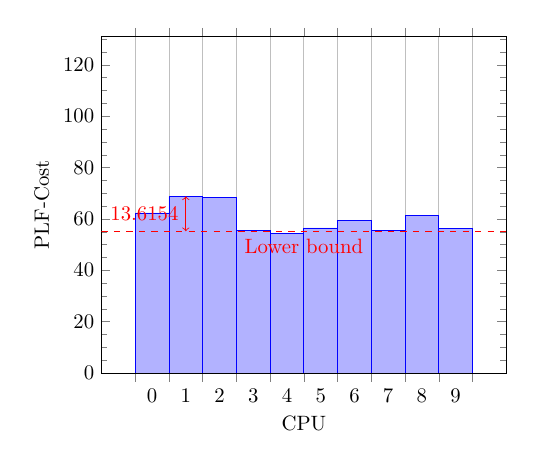
\begin{tikzpicture}[scale=0.75]
  \begin{axis}[ybar interval, ymax=130.949,ymin=0, minor y tick num = 3
, xlabel={CPU}, ylabel={PLF-Cost}]
    \addplot coordinates { (0,62.3052) (1,68.8015) (2,68.3548) (3,55.4615) (4,54.3747) (5,56.469) (6,59.3722) (7,55.4467) (8,61.4144) (9,56.3871) (10, 59.5223) };
\draw [red, dashed] ({rel axis cs:0,0}|-{axis cs:0,55.1861}) -- ({rel axis cs:1,0}|-{axis cs:10,55.1861}) node [pos=0.5, below] {Lower bound};
\draw [red, <->] ({axis cs:1.5,55.1861}) -- ({axis cs:1.5,68.8015}) node [pos=0.5, left] { 13.6154};
  \end{axis}
\end{tikzpicture}
\caption*{Weights repartition on the first tree}
\end{minipage}
\begin{minipage}{0.49\textwidth}
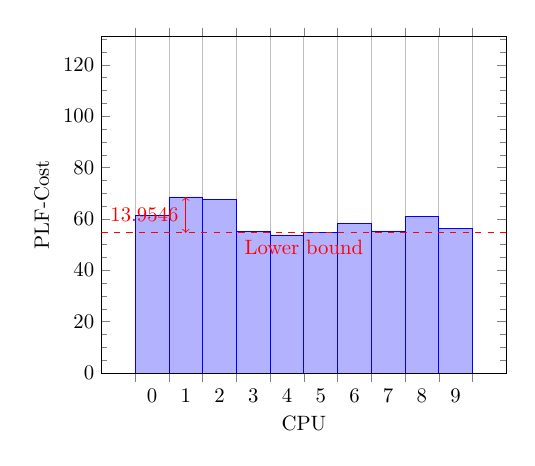
\begin{tikzpicture}[scale=0.75]
  \begin{axis}[ybar interval, ymax=130.949,ymin=0, minor y tick num = 3
, xlabel={CPU}, ylabel={PLF-Cost}]
    \addplot coordinates { (0,61.4938) (1,68.5434) (2,67.5112) (3,55.1439) (4,53.7494) (5,54.8784) (6,58.139) (7,55.3102) (8,60.8933) (9,56.3672) (10, 59.5223) };
\draw [red, dashed] ({rel axis cs:0,0}|-{axis cs:0,54.5888}) -- ({rel axis cs:1,0}|-{axis cs:10,54.5888}) node [pos=0.5, below] {Lower bound};
\draw [red, <->] ({axis cs:1.5,54.5888}) -- ({axis cs:1.5,68.5434}) node [pos=0.5, left] { 13.9546};
  \end{axis}
\end{tikzpicture}
\caption*{Weights repartition on the last tree}
\end{minipage}
\begin{minipage}{0.49\textwidth}
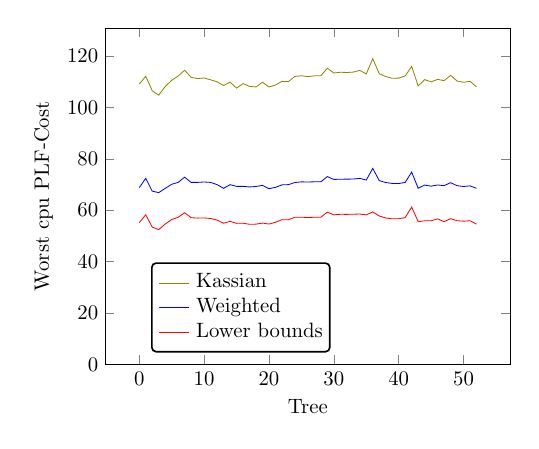
\begin{tikzpicture}[scale=0.75]
  \begin{axis}[ymax=130.949,ymin=0
, xlabel={Tree}, ylabel={Worst cpu PLF-Cost}]
    \addplot[mark=., color=blue] coordinates { (0,68.8015) (1,72.4392) (2,67.4516) (3,66.8685) (4,68.5211) (5,70.1365) (6,70.8536) (7,72.8933) (8,70.8511) (9,70.8561) (10,71.0174) (11,70.8486) (12,69.9777) (13,68.5459) (14,69.9628) (15,69.3052) (16,69.3201) (17,69.0769) (18,69.263) (19,69.6948) (20,68.3995) (21,68.9231) (22,69.8933) (23,69.9851) (24,70.8164) (25,71.0571) (26,71.0099) (27,71.0819) (28,71.072) (29,73.1141) (30,72.005) (31,72.1017) (32,72.1191) (33,72.1588) (34,72.4243) (35,71.7593) (36,76.2953) (37,71.5434) (38,70.8089) (39,70.4591) (40,70.4144) (41,70.8462) (42,74.8685) (43,68.5856) (44,69.8139) (45,69.3846) (46,69.8412) (47,69.6005) (48,70.7395) (49,69.5682) (50,69.2605) (51,69.5037) (52,68.5434) };
    \addplot[mark=., color=olive] coordinates { (0,109.122) (1,112.186) (2,106.529) (3,104.814) (4,108.201) (5,110.613) (6,112.29) (7,114.526) (8,111.754) (9,111.298) (10,111.514) (11,110.799) (12,110.02) (13,108.583) (14,109.916) (15,107.581) (16,109.323) (17,108.236) (18,108.022) (19,109.861) (20,108.007) (21,108.769) (22,110.196) (23,110.104) (24,112.124) (25,112.38) (26,112.052) (27,112.357) (28,112.397) (29,115.33) (30,113.462) (31,113.754) (32,113.653) (33,113.801) (34,114.486) (35,113.084) (36,119.045) (37,113.194) (38,112.094) (39,111.387) (40,111.474) (41,112.305) (42,116.062) (43,108.412) (44,110.881) (45,110.01) (46,110.978) (47,110.474) (48,112.533) (49,110.335) (50,109.824) (51,110.241) (52,108.03) };
    \addplot[mark=., color=red] coordinates { (0,55.1861) (1,58.2412) (2,53.4593) (3,52.4643) (4,54.639) (5,56.396) (6,57.2471) (7,59.0328) (8,57.1127) (9,56.9496) (10,57.0052) (11,56.7891) (12,56.1633) (13,54.9566) (14,55.6737) (15,54.906) (16,54.9576) (17,54.5208) (18,54.5965) (19,55.0027) (20,54.6313) (21,55.3151) (22,56.3404) (23,56.3114) (24,57.2628) (25,57.2871) (26,57.1806) (27,57.2777) (28,57.3005) (29,59.2752) (30,58.2298) (31,58.4323) (32,58.4022) (33,58.4496) (34,58.5494) (35,58.1886) (36,59.3677) (37,57.7799) (38,56.9923) (39,56.6655) (40,56.7151) (41,57.1266) (42,61.2583) (43,55.5739) (44,55.8935) (45,55.9017) (46,56.6467) (47,55.5551) (48,56.7179) (49,55.929) (50,55.7536) (51,55.9208) (52,54.5888) };
\node[draw=black,thick,rounded corners=2pt,above right=2mm] at (0, 0) {%
  \begin{tabular}{@{}r@{ }l@{}}
    \raisebox{2pt}{\tikz{\draw[olive] (0,0) -- (5mm,0);}}&Kassian\\
    \raisebox{2pt}{\tikz{\draw[blue] (0,0) -- (5mm,0);}}&Weighted\\
    \raisebox{2pt}{\tikz{\draw[red] (0,0) -- (5mm,0);}}&Lower bounds\\
  \end{tabular}};
  \end{axis}
\end{tikzpicture}
\caption*{Worst cpu weight for each tree with Kassian and with Weighted, and plot the lower bound for each tree}
\end{minipage}
